\section{Distributions}

\begin{frame}{Data Set}
    Let's consider some fundamental concepts and visualization techniques related to probability distributions using the following data set:
    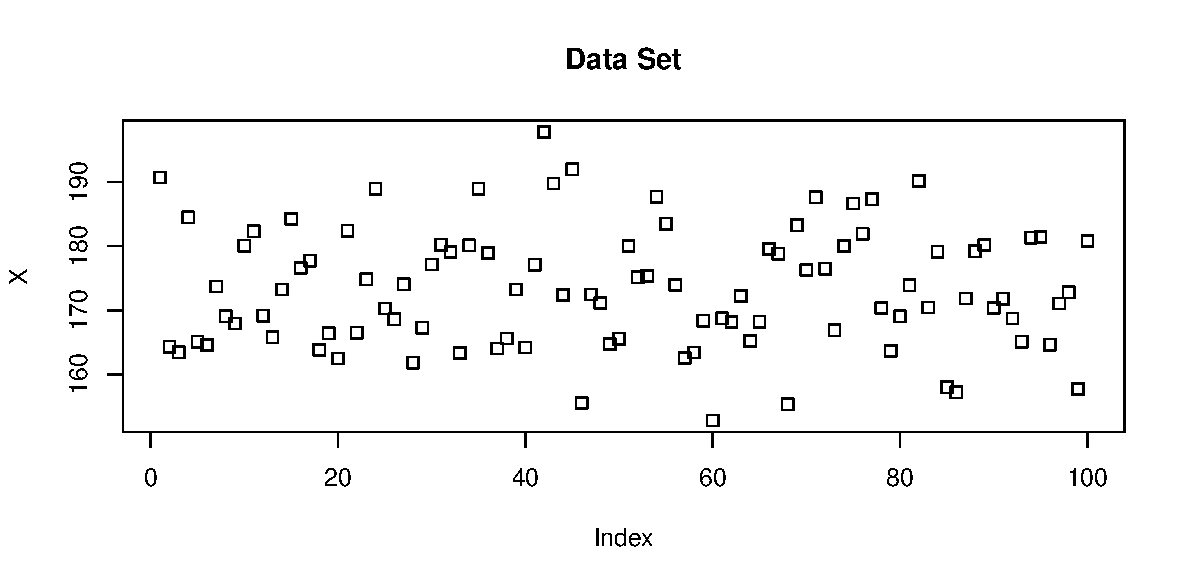
\includegraphics[width=\textwidth]{R/plots/distrib-data-set}
    The data can represent e.g. the height (cm) of 100 randomly selected people.

\end{frame}

\begin{frame}{Median}

    The \textbf{median} is the value separating an ordered data set into two equal parts. E.g. for a data set $\{1, 3, 5, 6, 7, 10, 11\}$ the median is 6.
    
    Let's see where the median and mean are located in our data set:
    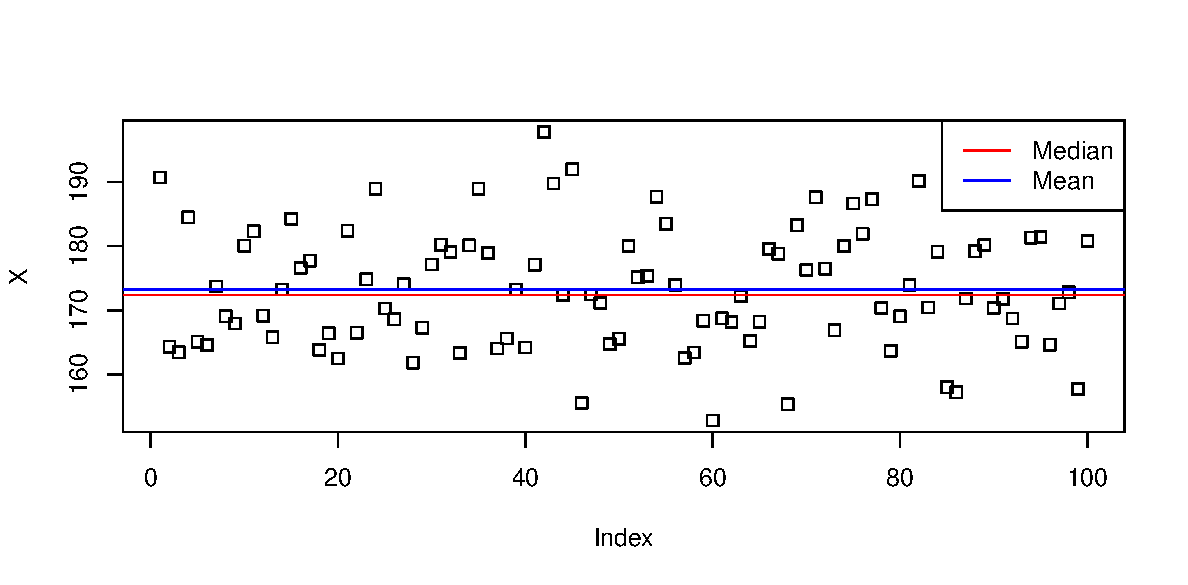
\includegraphics[width=\textwidth]{R/plots/distrib-median-vs-mean}

\end{frame}

\begin{frame}{Median}
    In the case the number of elements in the set is even, the median is calculated as the mean of the two middlemost numbers.
    
    \begin{example}
        \medskip
        \begin{itemize}
            \item What is the median for the set $\{1, 2, 5\}$?
            \item What is the median for the set $\{0, 1, 2, 5\}$?
            \item What is the median for the set $\{0, 1, 2, 100\}$?
        \end{itemize}
    \end{example}

    Answers: 2, 1.5, 1.5

\end{frame}

\begin{frame}{Histogram}

A histogram is an accurate graphical representation of the distribution of numerical data. E.g. for our data set it looks as follows:

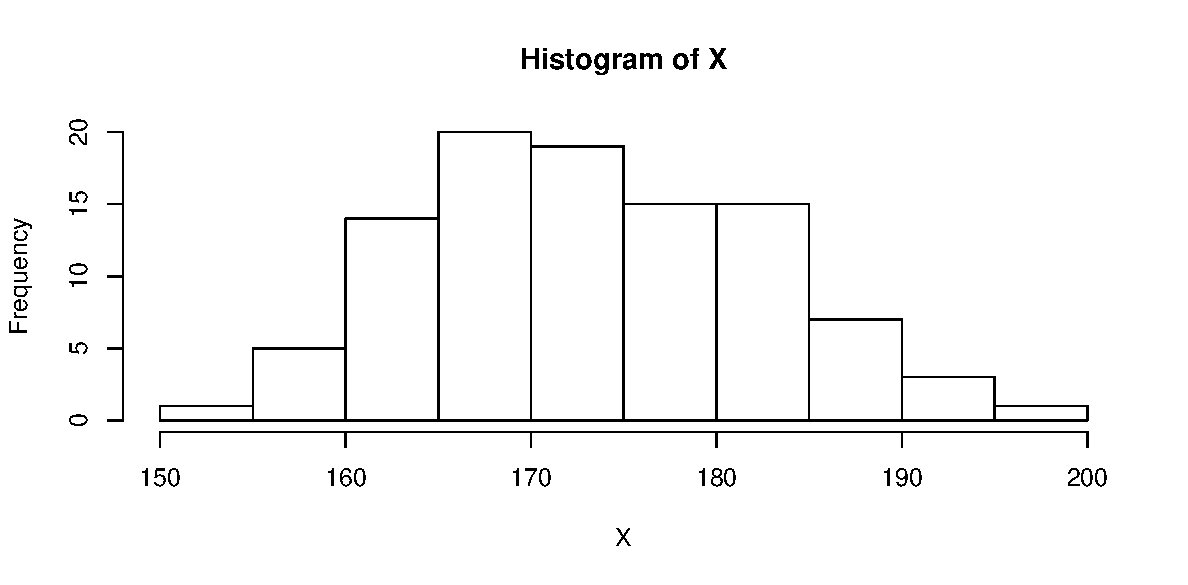
\includegraphics[width=\textwidth]{R/plots/distrib-histogram}

\end{frame}

\begin{frame}{Histogram}

The histogram plot depends on the chosen number of breaks:
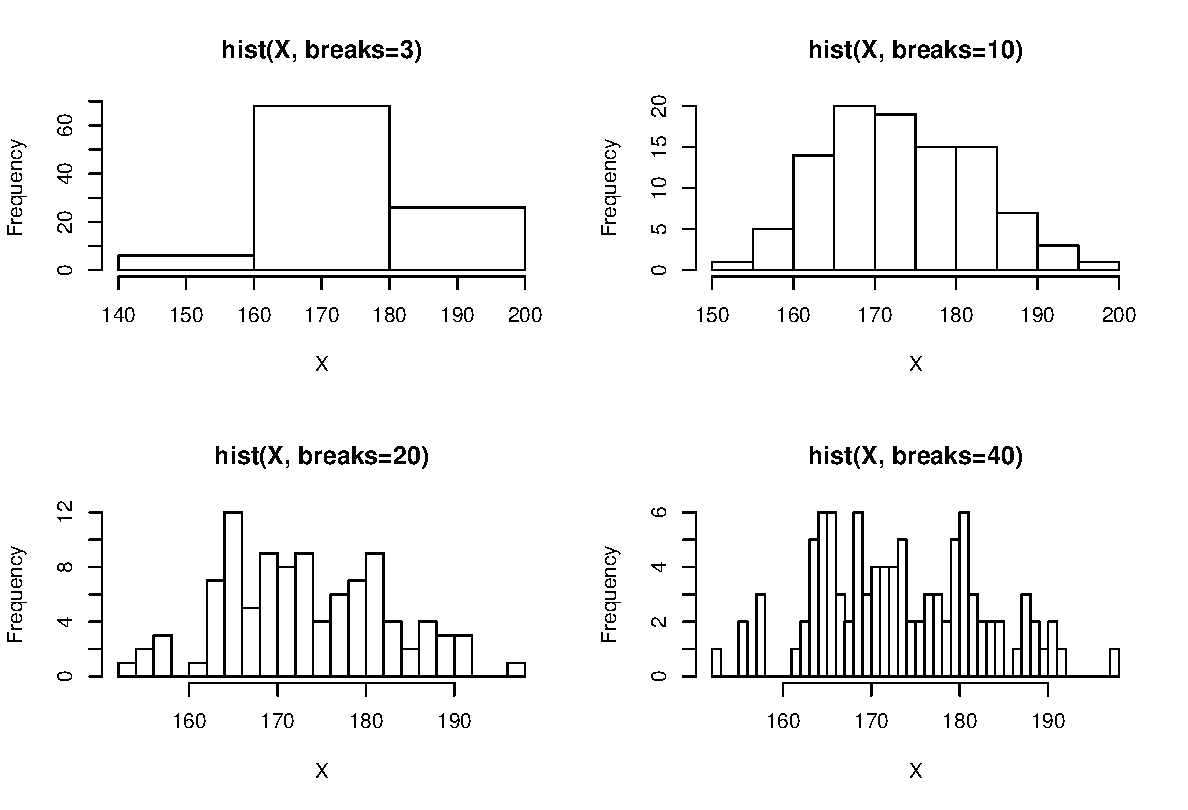
\includegraphics[width=\textwidth]{R/plots/distrib-histogram-bins}

\end{frame}

\begin{frame}{Quantile}

    The data set can be divided into groups of equal probability of occurring. The cut points used to generate these segments are called \textbf{quantiles}.
    
    $n$-quantiles divide the data set into $n$ groups. There are $n-1$ $n$-quantiles.
    
    E.g. the 4-quantiles (called \textbf{quartiles}) for our data set are Q1 = 165.72, Q2 = 172.40, Q3 = 180.02.
    
    Another way to look at it:

    \begin{table}
        \begin{tabular}{r r r r r}
            Min. & Q1 & Q2 & Q3 & Max. \\ \hline
            0\% & 25\%  & 50\% & 75\% & 100 \% \\ \hline
            152.81 & 165.72 & 172.40 & 180.02 & 197.80\\
        \end{tabular}
    \end{table}

    Note that Q2 is equivalent to median.

\end{frame}

\begin{frame}{Interquartile Range (IQR)}

    The \textbf{interquartile range (IQR)} is a measure of statistical dispersion, calculated as the difference of the upper and lower quartiles:
    
    \begin{equation*}
        IQR = Q3 - Q1 = 180.02 - 165.72 = 14.30
    \end{equation*}

    It is sometimes called \emph{middle 50\%}.

\end{frame}

\begin{frame}{PDF vs. CDF}

    If we integrate PDF over X, we will get a cumulative distribution function (CDF):
    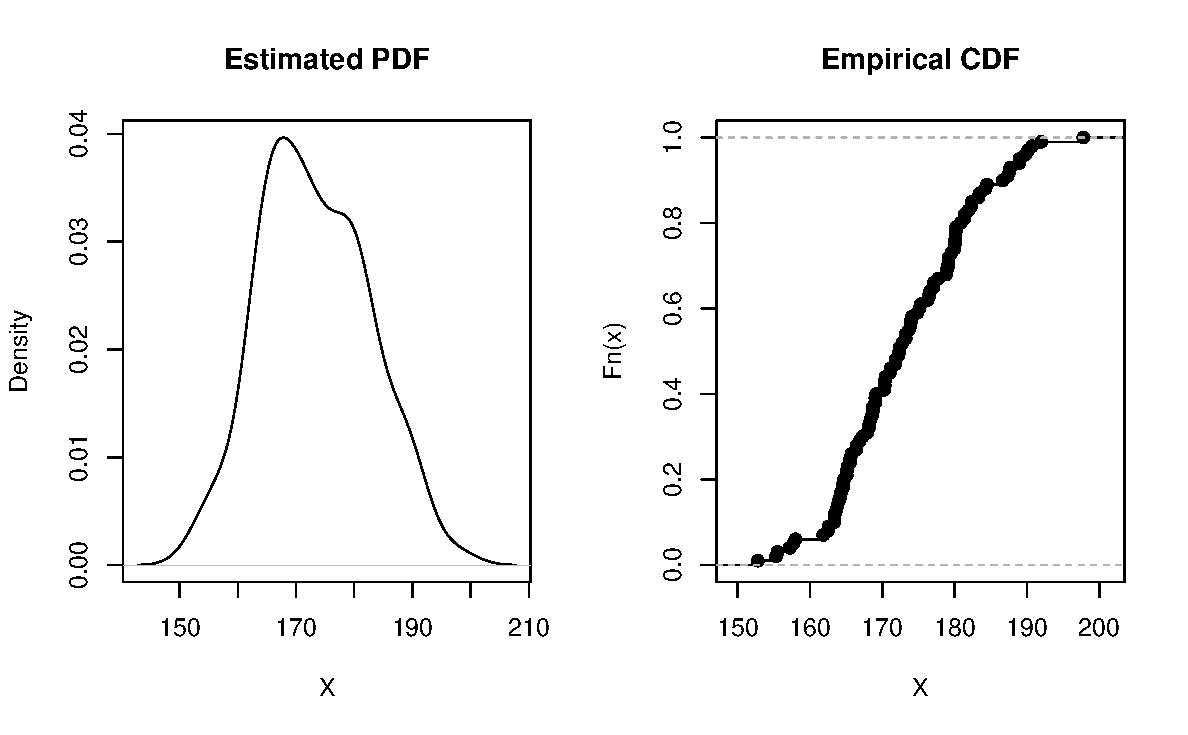
\includegraphics[width=\linewidth]{R/plots/distrib-pdf-vs-cdf}

\end{frame}

\begin{frame}{Quantile Function}
    The quantile function is the inverse of the cumulative distribution function:
    \begin{equation*}
    Q(p) = F(x)^{-1}
    \end{equation*}
    
    In other words, for a given $p$ it gives $x$ for which $P(X \leq x) = p$.
\end{frame}

\begin{frame}[fragile]{Hands-On Training: R}

    Plot a histogram, PDF, CDF and calculate the quartiles for the following data set:
    {\small
    \begin{verbatim}
    X <- rnorm(100)
    \end{verbatim}}

    You can use either \emph{R Base Graphics} or \emph{ggplot2}.
    
\end{frame}

\begin{frame}[fragile]{R Base Graphics}

    You may need these functions: {\small\texttt{plot, abline, hist, density, ecdf, quantile, summary, IQR}}.
    
    To draw subplots, you should first define the grid for subplots, e.g.:
    {\small
        \begin{verbatim}
        par(mfrow = c(2, 1)) # two rows, one column
        \end{verbatim}}
    \vspace{-15pt}
    Saving plots in R:
    {\small \url{https://www.stat.berkeley.edu/~s133/saving.html}}

\end{frame}

\begin{frame}{ggplot2}

    \begin{itemize}
        \item All data must be put into data frames or tibbles
        \item Find the corresponding plotting functions in the cheat sheet:\\ {\small\url{https://www.rstudio.com/wp-content/uploads/2015/03/ggplot2-cheatsheet.pdf}}
    \end{itemize}

\end{frame}

\begin{frame}{E(X) and Var(X) for Discrete Distribution}
    \begin{example}
        \medskip
        A random variable $X$ has the following distribution:
    
        \begin{tabular}{c|c|c|c|c|c}
            $x$      & 0   & 1   & 2   & 3   & 4   \\
            \hline
            $P(X=x)$ & 0.2 & 0.3 & 0.1 & 0.3 & 0.1
        \end{tabular}
    
        \begin{itemize}
            \item Draw the probability mass function.
            \item Calculate the expected value $E(X)$ and variance $Var(X)$.
        \end{itemize}
        \begin{align*}
        E(X) &= \sum_{i} p_i x_i\\
        Var(X) &= E[(X-E(X))^2] = \sum_{i} p_i (x_i - \mu)^2
        \end{align*}
    \end{example}
    % Answer: E(x) = 1.8, Var(x) = 1.76

\end{frame}

\begin{frame}{Parametric Family of Distributions}

    \begin{columns}
    \begin{column}{0.5\textwidth}
        {\small
        \begin{itemize}
            \item Probabilities often depend on some numerical constants
            \item In such cases, it is possible to parametrize the PDF
            \item In other cases, parametric distributions can be used as good approximations
            \item Examples of parametric distributions that are used very often:
            \begin{enumerate}
                \item binomial distribution
                \item geometric distribution
                \item normal distribution
            \end{enumerate}
        \end{itemize}
        }
    \end{column}
    \begin{column}{0.5\textwidth}
         \begin{figure}
             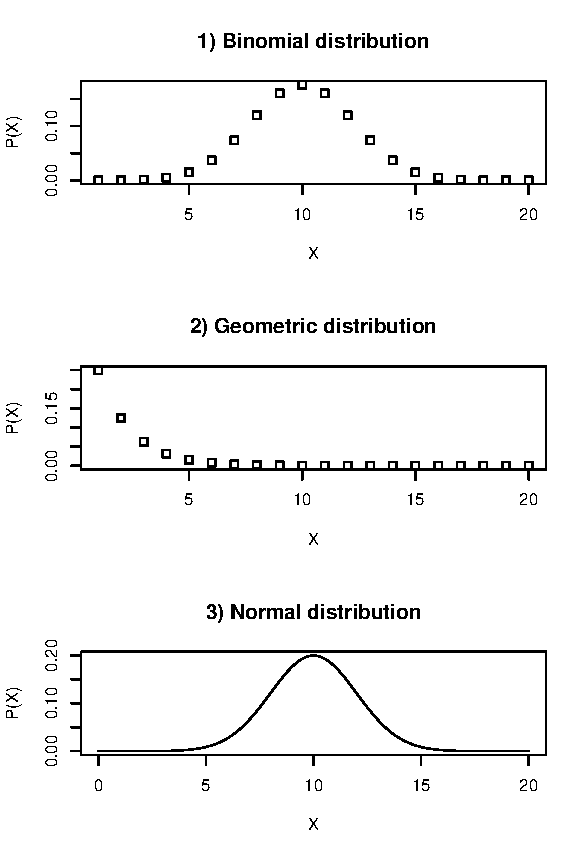
\includegraphics[width=\textwidth]{R/plots/distributions}
         \end{figure}
    \end{column}
    \end{columns}

\end{frame}

\begin{frame}{Bernoulli Distribution}

    It is a distribution with just two possible outcomes, 0 and 1.
    
    Its PMF can be expressed as follows:
    \begin{equation}
    f(k, p) = P(X = k) =
    \begin{cases}
    q = (1 - p) & \text{for } k = 0\\
    p           & \text{for } k = 1
    \end{cases}
    \end{equation}
    
    Alternatively:
    \begin{equation}
    f(k, p) = P(X = k) = p^k (1-p)^{1-k} \text{ for } k \in \{0, 1\}
    \end{equation}

    

\end{frame}

\begin{frame}{Binomial Distribution}

    \begin{columns}
    \begin{column}{0.25\textwidth}
        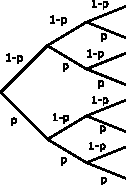
\includegraphics[width=\linewidth]{gfx/probability_tree}
    \end{column}
    \begin{column}{0.75\textwidth}
        \begin{example}
            \medskip
            The probability of a success in some trial is $p=0.3$. Consider an experiment with 3 independent trials ($n=3$). Calculate the probabilities that there will be exactly:
            \begin{itemize}
                \item 1 success $\rightarrow P(1) = 3p(1-p)^2$
                \item 2 successes $\rightarrow P(2) = 3p^2(1-p)$
                \item 3 successes $\rightarrow P(2) = p^3$
            \end{itemize}
            How would you calculate it for $n=100$?
        \end{example}
    \end{column}
    \end{columns}

\end{frame}

\begin{frame}{Binomial Distribution}
    The probability of getting $k$ successes in $n$ trials is given by:
    \begin{equation}
    f(k, n, p) = P(X = k) = \binom{n}{k} p^k (1 - p)^{n-k}
    \end{equation}
    where $p$ is the probability of a success in a single trial.
    
    $\binom{n}{k}$ is the binomial coefficient, read as ``$n$ choose $k$", and calculated as follows:
    \begin{equation}
    \binom{n}{k} = \frac{n!}{(n - k)! k!}
    \end{equation}
    
    $\binom{n}{k}$ is equal to the number of subsets of size $k$ that can be formed from a group of $n$ distinct items.
\end{frame}

\begin{frame}{Binomial Coefficient}
    \begin{example}
        \medskip
        How many subsets of size 2 can be selected from the set \{1, 2, 3, 4\}? List all subsets, then calculate by hand and compare with R.
    \end{example}

    \begin{shownto}{teacher}
        Answer: 6
    \end{shownto}

    {\tiny R command: \texttt{choose(n, k)}}
\end{frame}

\begin{frame}{Binomial Distribution}
    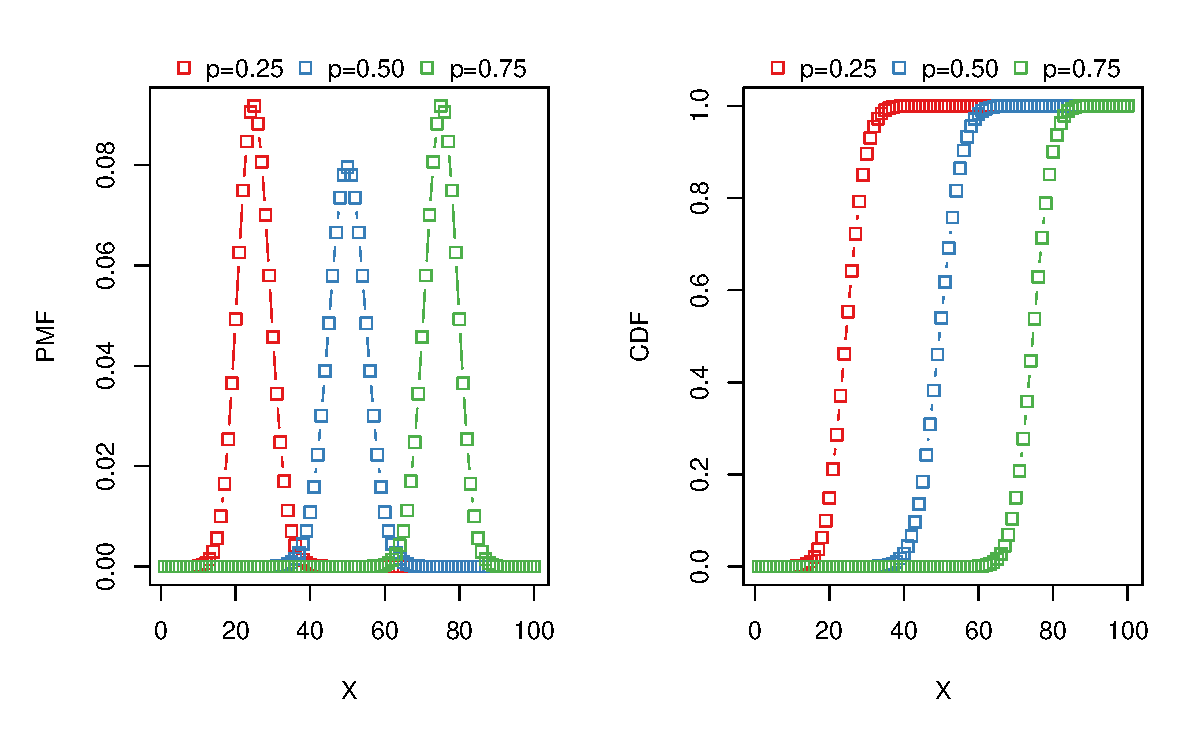
\includegraphics[width=\linewidth]{R/plots/binomial-distribution}

    {\tiny R commands: \texttt{dbinom}, \texttt{pbinom}, \texttt{qbinom}, \texttt{rbinom}}
\end{frame}

\begin{frame}{Binomial Distribution}
    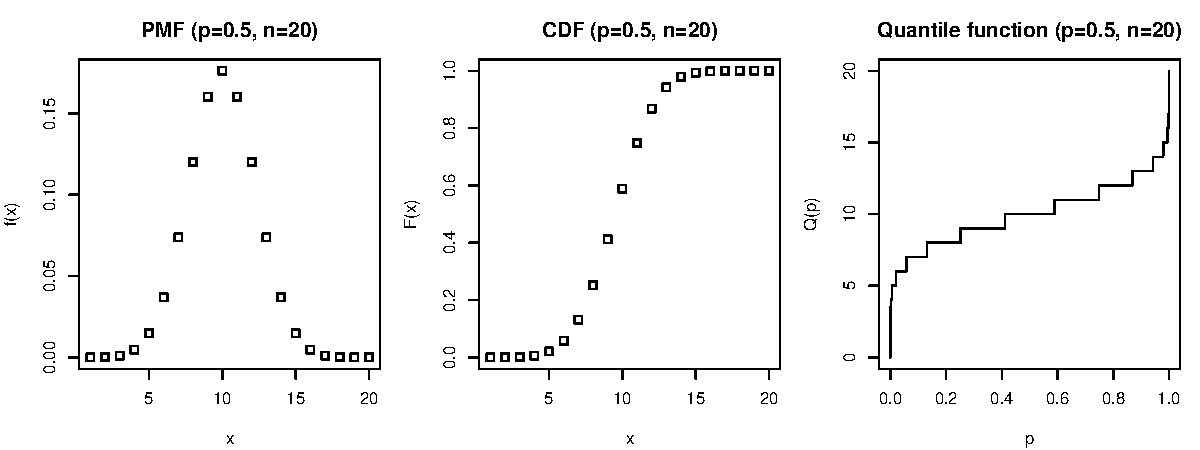
\includegraphics[width=0.95\linewidth]{R/plots/density-cumulative-quantile}
    \begin{itemize}
        \item \textbf{PMF:} What is the probability that there will be $X=k$ successes? $\rightarrow f(x) = P(X=k)$
        \item \textbf{CDF:} What is the probability that there will be less or equal than $X=n$ successes? $\rightarrow F(x) = P(X \leq k)$
        \item \textbf{QF:} What is the number of successes such that the probability of getting this number or less is $p$? $\rightarrow Q(p) = F^{-1}(x)$
    \end{itemize}
\end{frame}

\begin{frame}{Binomial Distribution}
    \begin{example}
        \medskip
        \begin{itemize}
            \item Plot binomial distribution density experimenting with different $n$ (number of trials) and $p$ (probability of success per trial).
            \item How to calculate the most probable value of $k$ (expected number of successes) in each case?
        \end{itemize}
    \end{example}
\end{frame}

\begin{frame}{Binomial Distribution}

    \begin{example}
        \medskip
        Draw a target on the blackboard and play the ``paper cannon" game (rules to be explained during the lecture). Based on 10 trials, estimate the chance of success in hitting the target. \begin{itemize}
            \item Calculate the probability that a person would hit the target at least 20 times in 100 trials.
            \item Calculate the probability that a person would miss the target more than 20 times in 100 trials.
            \item Calculate the probability $P(X = 100)$ for $n = 100$.
            \item What is the number of successes $k$ in 100 trials, so that $P(X > k) = 90\%$.
        \end{itemize} 
        
        {\tiny Hint: Use CDF and the quantile function of the binomial distribution.}
    \end{example}

\end{frame}

\begin{frame}{Binomial Distribution}
\begin{example}
    \medskip
    Draw a target on the blackboard and play the ``paper cannon" game (rules to be explained during the lecture). Based on 10 trials, estimate the chance of success in hitting the target. Subsequently, calculate the probability that a person would miss the target more than 20 times in 100 trials.
    
    {\tiny Hint: Use CDF of the binomial distribution}
\end{example}
\end{frame}

\begin{frame}{Geometric Distribution}

    The \textbf{geometric distribution} describes the probability that a given trial is the first one successful in a series of trials.
    
    \emph{There are two possible definitions.} The probability that the $k$th trial is the first success is given by Eq.~(\ref{pgeomk1}). The probability that there will be $k$ failures before the first success is given by Eq.~(\ref{pgeomk0}).
    \begin{align}
    P(X=k) &= (1-p)^{k-1} p,\quad k=1, 2, 3, ...\label{pgeomk1}\\
    P(X=k) &= (1-p)^k p,\quad k=0, 1, 2, ...\label{pgeomk0}
    \end{align}
    
    Eq.~(\ref{pgeomk0}) is used in R functions: {\small \texttt{dgeom}, \texttt{pgeom}, \texttt{qgeom}, \texttt{rgeom}}.
\end{frame}

\begin{frame}{Geometric Distribution}
    \begin{columns}
    \begin{column}{0.25\textwidth}
        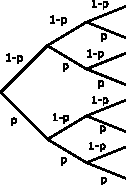
\includegraphics[width=0.9\linewidth]{gfx/probability_tree}
    \end{column}
    \begin{column}{0.75\textwidth}
        \begin{example}
            \medskip
            Calculate the probabilities that:
            \begin{itemize}
                \item the 1st trial is the first success
                \item the 2nd trial is the first success
                \item the 3rd trial is the first success
            \end{itemize} 
        \end{example}
    \end{column}
    \end{columns}
\end{frame}

\begin{frame}{Geometric Distribution}
    Number of failures before the first success, based on Eq.~(\ref{pgeomk0}):
    
    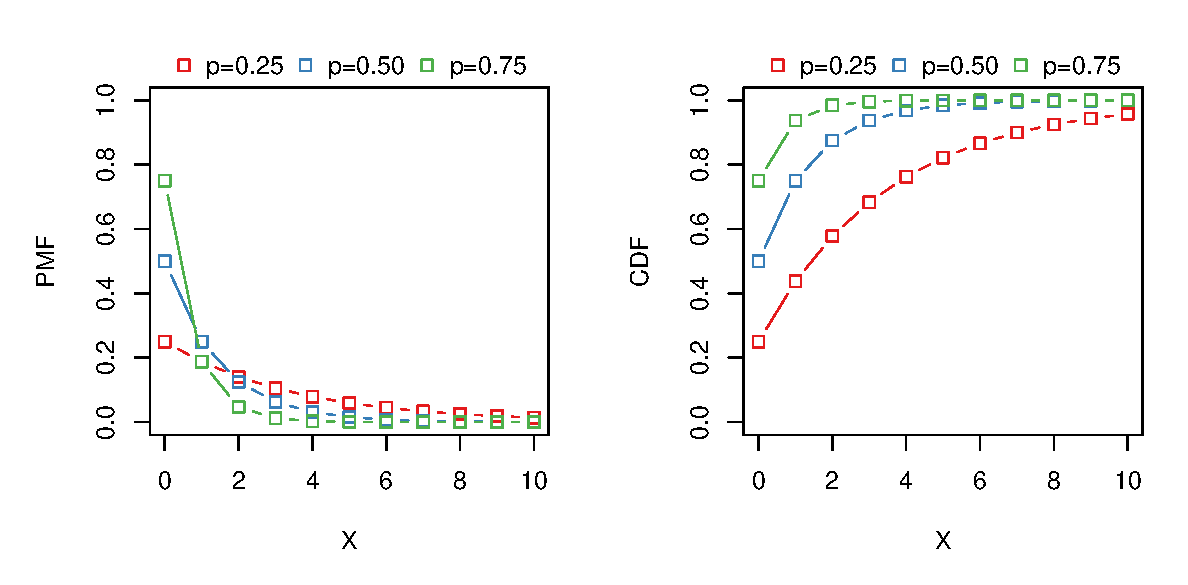
\includegraphics[width=\linewidth]{R/plots/geometric-distribution}
    
    {\tiny R commands: \texttt{dgeom}, \texttt{pgeom}, \texttt{qgeom}, \texttt{rgeom}}
\end{frame}

\begin{frame}{Geometric Distribution}
    \begin{example}
        \medskip
        Given $p=0.3$, calculate the following:
        \begin{itemize}
            \item $P(X \leq 4)$
            \item $P(X=10)$
            \item Find $k$ such that $P(X \leq k) = 0.5$.
            \item How many trials are needed to be 90\% sure we get at least one success?
        \end{itemize}
    
        {\tiny Hint: The number of trials needed to get at least one success is one larger than the number of preceding failures.}
    \end{example}
\end{frame}

\begin{frame}{Poisson Distribution}

    The \textbf{Poisson distribution} is a discrete probability distribution (like binomial and geometric), expressing the probability of a given number of events $k$ occurring in a fixed interval of time. It's assumed that the events occur at a constant rate $\lambda$. 
    
    \begin{equation}
    P(X=k) = \frac{\lambda ^ k e ^{-\lambda}}{k!}
    \end{equation}

    Examples:
    \begin{itemize}
        \item the number of phone calls received by a call center per hour
        \item the number of computer technical failures in a data center per week
    \end{itemize}
    
\end{frame}

\begin{frame}{Poisson Distribution}

    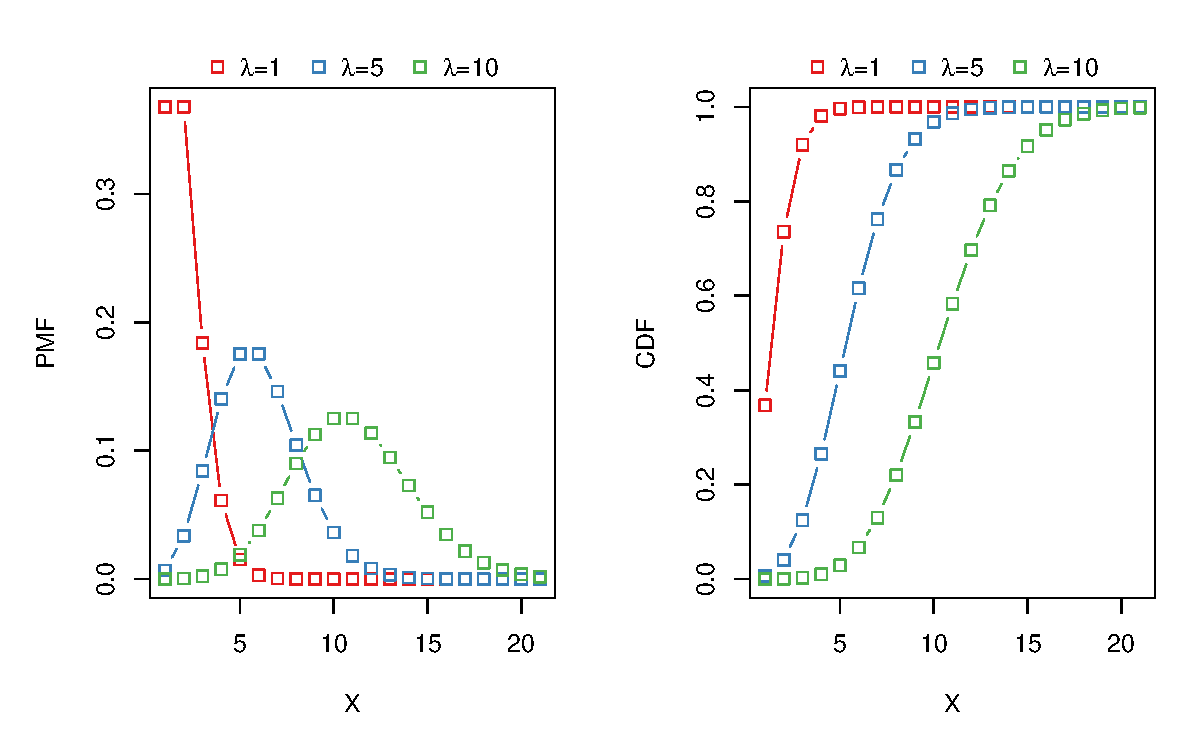
\includegraphics[width=\linewidth]{R/plots/poisson-distribution}
    {\tiny R commands: \texttt{dpois}, \texttt{ppois}, \texttt{qpois}, \texttt{rpois}}

\end{frame}

\begin{frame}{Conditions For Poisson Distribution}
\label{}

\textbf{The following conditions have to be met to use this distribution:}
\begin{itemize}
\item Events can occur any number of times during a time period
\item Events occur independently
\item Events occur at a constant rate
\item The probability of an event is proportional to the length of the time period
\end{itemize}

\end{frame}

\begin{frame}{Poisson Distribution}
    \begin{example}
        \medskip
        In a data center computer failures occur at an average rate of 100 per week.
        
        (a) What is the probability that the number of failures next week will be less than 80?
        
        \begin{equation*}
        P(X < 80) = P(0, 1, 2, ..., 79) = \sum_{i=0}^{79} P(i)
        \end{equation*}
        
        Calculate in R using: (1) \texttt{for} loop, (2) \texttt{ppois} function.
        
        (b) What is the probability $P(X = 100)$?
    \end{example}
\end{frame}

\begin{shownto}{teacher}
    \begin{frame}{Poisson Distribution vs. Binomial Distribution}
    With respect to the point (a) from the previous example, explain the following:
    \vspace{10pt}
    
    $0.99^{100}$ = \\
    {\small\texttt{ppois(0, lambda=1)}} = \\
    {\small\texttt{dbinom(0, size=100, prob=0.01)}} = \\
    {\small\texttt{dbinom(100, size=100, prob=0.99)}}
    \vspace{10pt}
    
    \pause
    Do you see now, where the conditions for using Poisson distribution come from?
    \end{frame}
\end{shownto}

\begin{frame}{Poisson Distribution}
    \begin{example}
        \medskip
        A one-hundred-year flood is a flood event that has a 1\% probability of occurring in any given year.
        \begin{itemize}
            \item What is the probability that there will be no one-hundred-year flood within the next 100 years?
            \item What is the number of floods $k$ so that $P(X > k) = 1\%$?
        \end{itemize}
        Does the answer change if the last flood occurred just one year ago?
    \end{example}
\end{frame}

\begin{frame}{Normal Distribution}

    The \textbf{normal (Gaussian) distribution} is arguably the most often used probability distribution in statistics. It is a continuous distribution.
    
    It is defined with two parameters: mean $\mu$ and standard deviation $\sigma$ (or variance $\sigma^2$). If a random variable $X$ is normally distributed, we write $X \sim \mathcal{N}(\mu, \sigma)$.
    
    \begin{equation}
    f(x) = \frac{1}{\sqrt{2\pi\sigma^2}} e ^{-\frac{(x - \mu)^2}{2\sigma^2}}
    \end{equation}
    
    If $\mu = 0$ and $\sigma = 1$, the function is often referred to as the \emph{standard normal distribution}: $f(x|\mu=0,\sigma=1) = \frac{1}{\sqrt{2\pi}} e ^{-0.5 x^2}$

\end{frame}

\begin{frame}{Normal Distribution}
    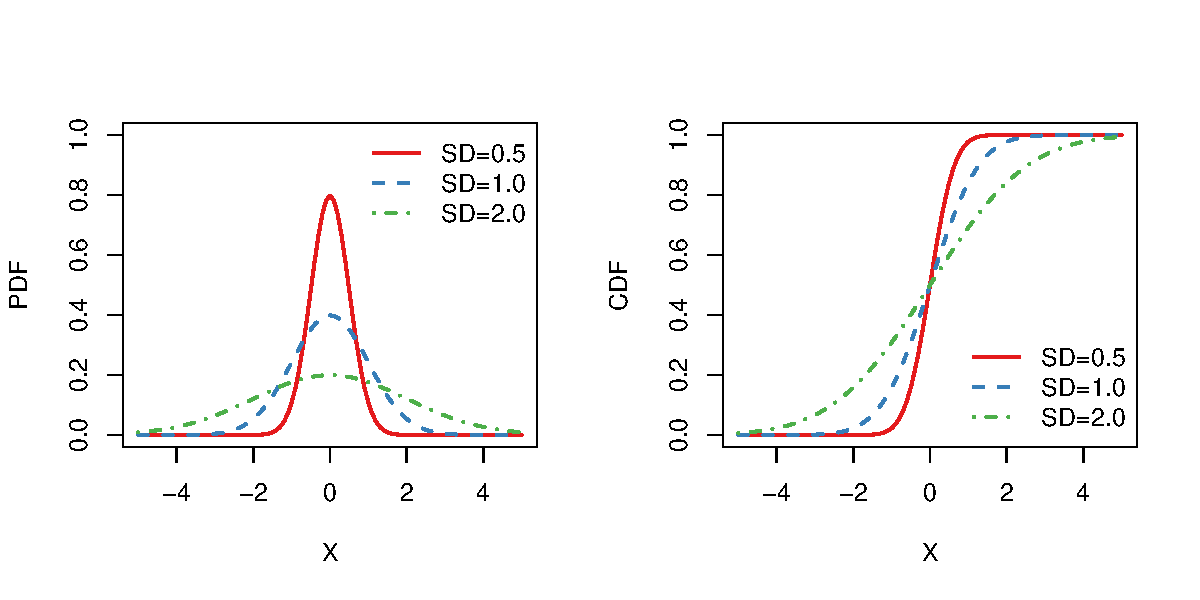
\includegraphics[width=\linewidth]{R/plots/normal-distribution}
    \begin{example}
        \medskip
        Calculate $P(X > 0.5)$ and $P((X > 0.5) \cup (X < -0.5))$ if $X \sim \mathcal{N} (\mu = 0, \sigma = 0.5)$
    \end{example}

    {\tiny R commands: \texttt{dnorm}, \texttt{pnorm}, \texttt{qnorm}, \texttt{rnorm}}
\end{frame}

\begin{frame}{Normal Distribution}

    \begin{example}
        \medskip
        Run the following code:
        
        \texttt{curve(exp(-x\^{}2), from = -3, to = 3)}
        
        Discuss the meaning of the parameters and scaling factors in the normal distribution: $\sqrt{\pi}, \frac{1}{2}, \sigma^2, \mu$.
        
        \begin{align*}
        f(x) &= \frac{1}{\sqrt{2\pi\sigma^2}} e ^{-\frac{(x - \mu)^2}{2\sigma^2}} \\
        f(x|\mu=0,\sigma=1) &= \frac{1}{\sqrt{2\pi}} e ^{-\frac{1}{2} x^2}
        \end{align*}
    \end{example}

\end{frame}

\begin{frame}{Normal Distribution: 68-95-99.7 Rule}

    \begin{figure}
        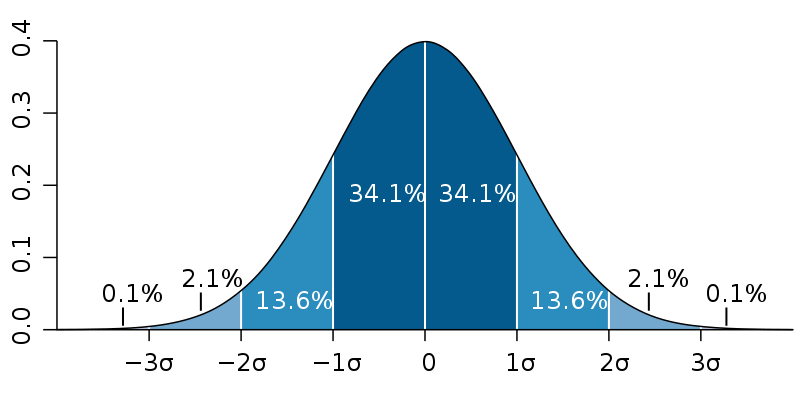
\includegraphics[width=0.7\linewidth]{gfx/web/standard-deviation-diagram}
    \end{figure}
    \begin{align*}
    P(\mu - 1\sigma \leq X \leq \mu + 1\sigma) &\approx 0.68 \\
    P(\mu - 2\sigma \leq X \leq \mu + 2\sigma) &\approx 0.95 \\
    P(\mu - 3\sigma \leq X \leq \mu + 3\sigma) &\approx 0.997 \\
    \end{align*}
    
    {\tiny Image: \url{https://commons.wikimedia.org/wiki/File:Standard_deviation_diagram.svg}}

\end{frame}

\begin{frame}{Normal Distribution}
    \begin{example}
        \medskip
        Consider a random variable $X \sim \mathcal{N}(\mu=0, \sigma=1)$.
        \begin{itemize}
            \item What is the probability $P(X=0)$?
            \item What is the probability $P(-1 < X < 1)$?
            \item What is the probability $P((X < -3) \cup (X > 3))$?
            \item What is the probability $P(X > 3)$?
        \end{itemize}
    \end{example}
\end{frame}

\begin{frame}{Evaluating the Normal Approximation}

    \begin{figure}
        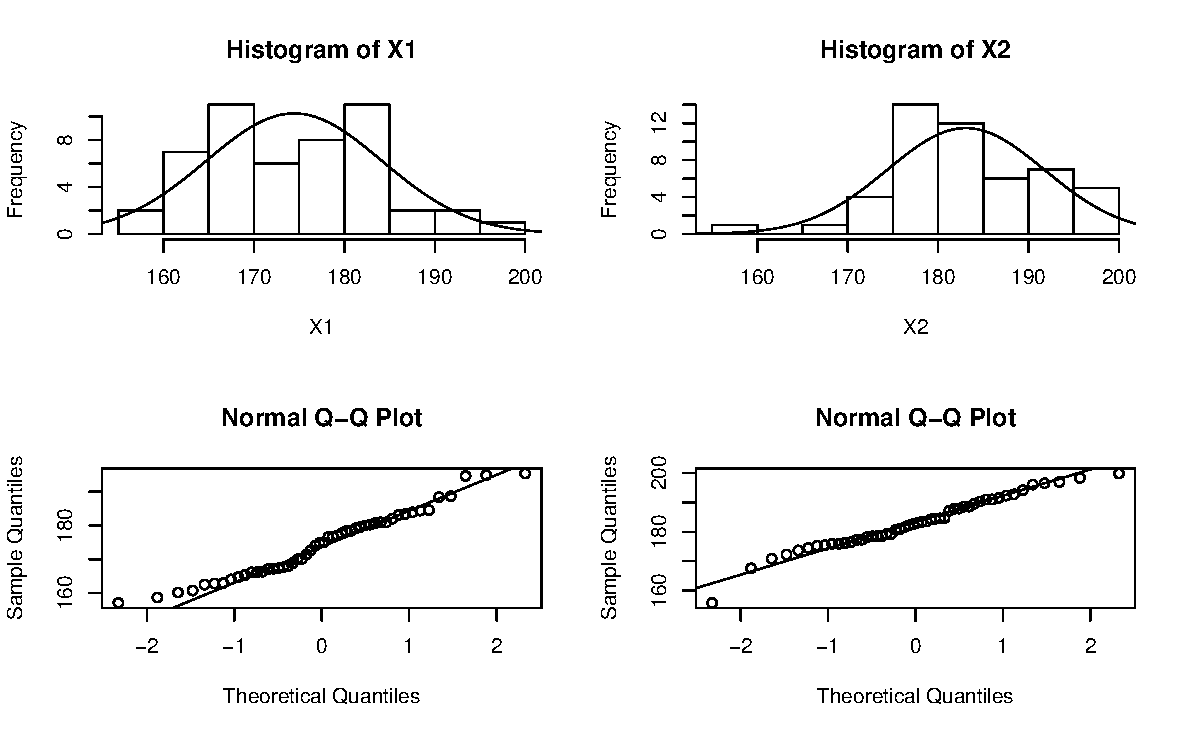
\includegraphics[width=\linewidth]{R/plots/eval_norm_approx}
    \end{figure}

    {\tiny R commands: \texttt{hist}, \texttt{qqnorm}, \texttt{qqline}}

\end{frame}

\begin{frame}[fragile]{Evaluating the Normal Approximation: R Code}

    {\tiny
    \begin{verbatim}
        # Exemplary data sets
        X1 <- rbeta(50, shape1 = 3, shape2 = 5) * 60 + 150
        X2 <- rnorm(50, mean = 180, sd = 10)

        # Plot
        windows(width = 8, height = 5)
        par(mfrow = c(2, 2))

        h <- hist(X1)
        mlp <- mean(h$counts / h$density) # Multiplier for the norm. dist. func.
        xn <- seq(150, 210, by = 0.1)
        yn <- dnorm(xn, mean = mean(X1), sd = sd(X1))
        lines(xn, yn * mlp, type = 'l')
        
        hist(X2)
        mlp <- mean(h$counts / h$density) # Multiplier for the norm. dist. func.
        xn <- seq(150, 210, by = 0.1)
        yn <- dnorm(xn, mean = mean(X2), sd = sd(X2))
        lines(xn, yn * mlp, type = 'l')
        
        qqnorm(X1)
        qqline(X1)
        
        qqnorm(X2)
        qqline(X2)
    \end{verbatim}
    }

\end{frame}

\begin{frame}{Normal Distribution}
    \begin{example}
        \medskip
        Take three samples from a normal distribution: $N_1 = 10$, $N_2 = 30$, $N_3 = 100$. Evaluate the normal approximation for each sample. What is the conclusion with respect to the sample size?
    \end{example}
\end{frame}

\begin{frame}{Normal Distribution}
    \begin{example}
        \medskip
        Take an anonymous sample of the height of SDU students:\\
        \url{http://bit.ly/sta2018-height}
        
        Tasks:
        \begin{itemize}
            \item Evaluate the normal approximation.
            \item What is the probability to observe a person higher than 2m?
        \end{itemize}
    \end{example}
\end{frame}

\begin{frame}{Binomial Distribution: Normal Approximation}
    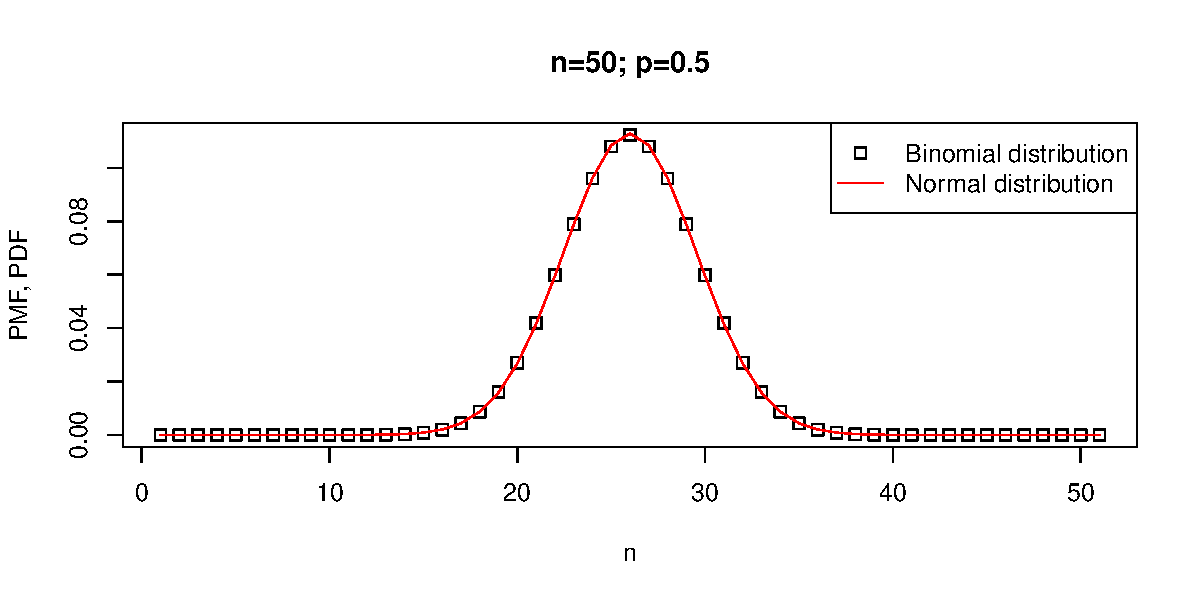
\includegraphics[width=\linewidth]{R/plots/norm_approx_to_binom}
    For large $n$ and $p$ not too far from 0.5 the binomial distribution can be approximated with the normal distribution:
    $\mathcal{N}\left( \mu = np, \sigma = \sqrt{np(1-p)} \right)$.
\end{frame}

\begin{frame}{Binomial Distribution: Normal Approximation}
    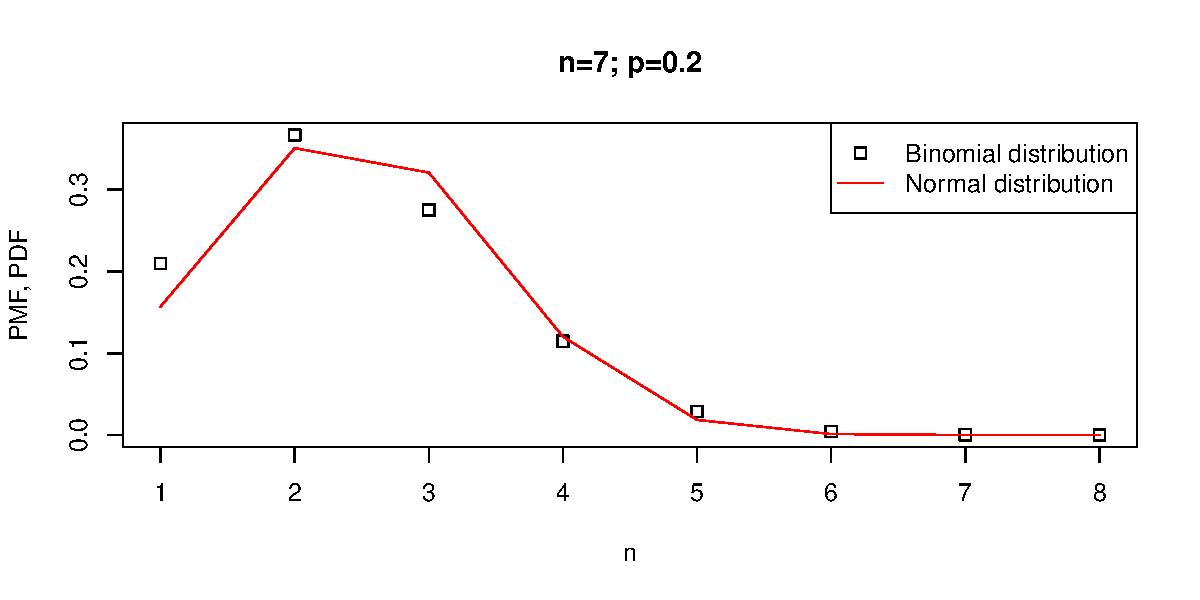
\includegraphics[width=\linewidth]{R/plots/norm_approx_to_binom_2}
    The approximation is not accurate for small $n$, especially if $p$ is far from 0.5.
\end{frame}

\begin{frame}{t-Distribution}

    If the sample size is small ($n < 30$) and the population standard deviation is unknown, we often use the t-distribution instead of the normal distribution. t-distribution depends only on the number of degrees of freedom $df = n - 1$. For $df \ge 30$ it's almost indistinguishable from the standard normal distribution.
    
    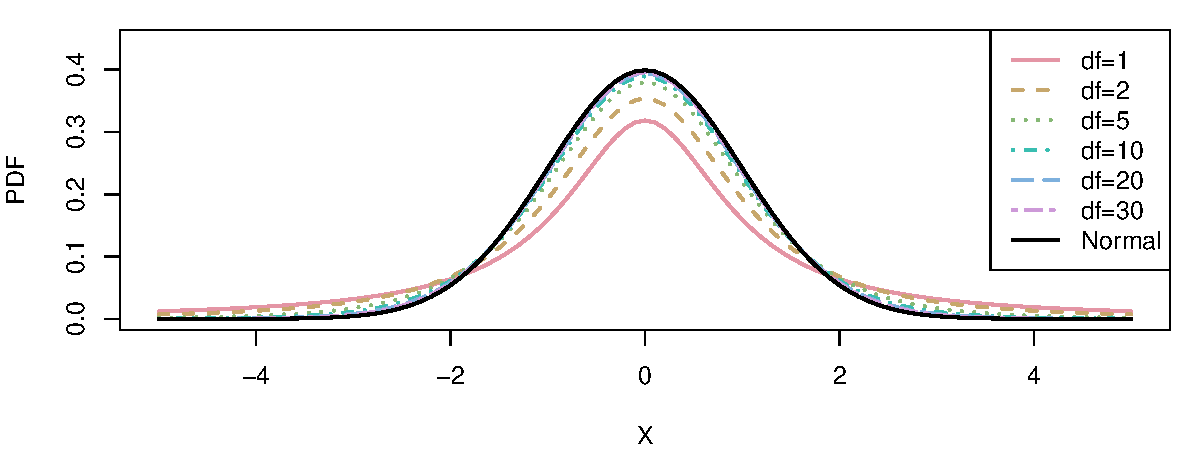
\includegraphics[width=\linewidth]{R/plots/t_distribution}
    {\tiny R commands: \texttt{dt}, \texttt{pt}, \texttt{qt}, \texttt{rt}}

\end{frame}

\begin{frame}{Degrees of Freedom: Intuitive Explanation}
   
    Imagine you have 4 unknown numbers ($a , b , c , d$) with the mean equal to 20:
    \begin{equation*}
    \frac{a + b + c + d}{4} = 20.
    \end{equation*}
    
    We can arbitrarily suggest 3 numbers ($a, b, c$), but the last number ($d$) is not free - there is only one specific $d$ satisfying the overall mean of 20.
    
    In general, the degrees of freedom is equal to the number of observations minus the number of parameters to be estimated (e.g. means).
    
    \begin{example}
        \medskip
        If $x_1 = 0$, choose $x_2$ and $x_3$ so that $\mu_{x} = 0$ and $\sigma^2_{x} = 1$.
        %Answer depends on the denominator (N or N-1). If N then x2 = -1.22, x3 = 1.22, if N-1 then x2 = -1, x3 = 1.
    \end{example}
    
\end{frame}

\begin{frame}{Hands-On Training: R}
    
    TutorialsPoint:
    \begin{itemize}
        \item \url{https://www.tutorialspoint.com/r/r_decision_making.htm}
        \item \url{https://www.tutorialspoint.com/r/r_loops.htm}
    \end{itemize}

    R for Data Science:
    \begin{itemize}
        \item \url{http://r4ds.had.co.nz/transform.html}
    \end{itemize}

    \begin{itemize}
        \item \url{http://r4ds.had.co.nz/exploratory-data-analysis.html}
        \item \url{http://r4ds.had.co.nz/workflow-projects.html}
    \end{itemize}

\end{frame}

\begin{frame}{Hands-On Training: R}

    R for Data Science:
    \begin{itemize}
        \item \url{http://r4ds.had.co.nz/exploratory-data-analysis.html}
        \item \url{http://r4ds.had.co.nz/workflow-projects.html}
    \end{itemize}

\end{frame}
